\documentclass{beamer}
\usetheme{Singapore}
%\setbeamercolor{structure}{fg=red}
\usepackage{upgreek}
\usepackage{color}
%\def\magyarOptions{hyphenation=huhyphn}
%\usepackage{ae,aecompl}
%\usepackage[T1]{fontenc}
\usepackage[utf8]{inputenc}
%\usepackage[hungarian]{babel}
\usepackage{gensymb}
\usepackage{pgfplots}
\usepackage{pst-plot}
\usepackage{tikz}
\usepgfplotslibrary{external}
\tikzexternalize
\usepackage[version=3]{mhchem}

\normalfont
\title{A Belouszov‐Zsabotyinszkij reakció térképezése pásztázó elektrokémiai mikroszkóppal}
\subtitle{Analitikai Napok 2018, Balatonszemes}
\author
{Kiss András\\
\hfill \\
}
\institute
{
  %\inst{1}%
  Általános és Fizikai Kémia Tanszék\\
  Pécsi Tudományegyetem\\
  \hfill \\

  \includegraphics[width=0.14\textwidth]{pte_logo.eps}\\
  2018. április 23-24
}

\date[]

\begin{document}
\frame{\titlepage}  


\begin{frame}
	\centering
	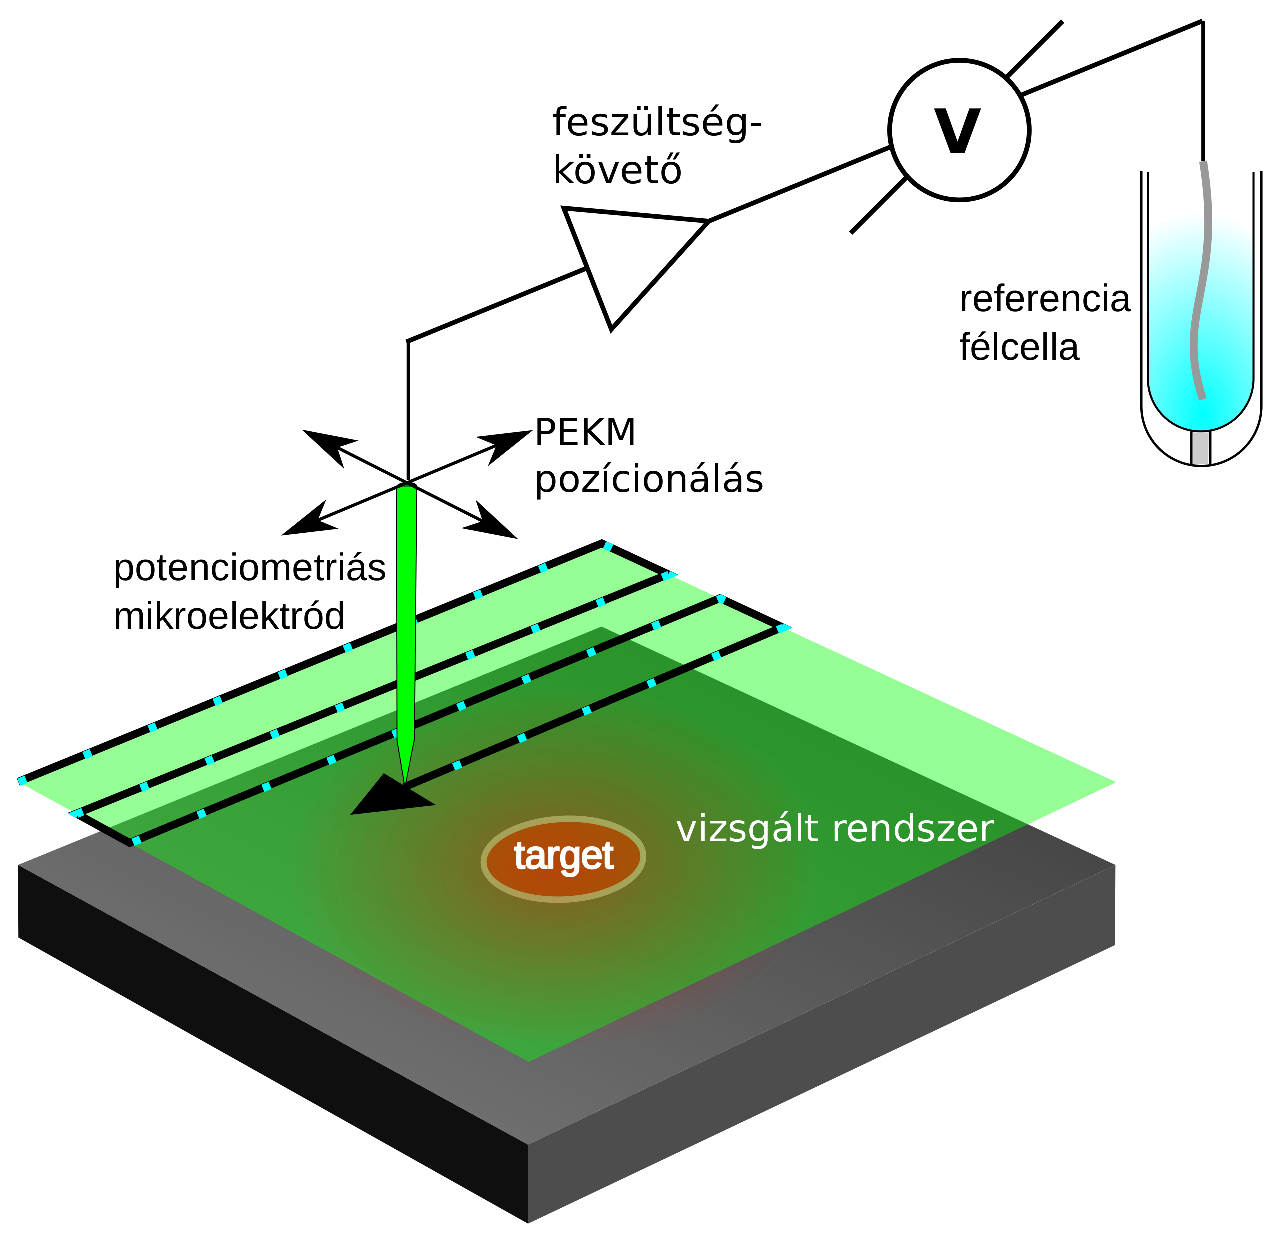
\includegraphics[width=0.6\textwidth]{secm.eps}
	\frametitle{\underline{P}ásztázó \underline{E}lektro\underline{k}émiai \underline{M}ikroszkóp}
\end{frame}

\begin{frame}
	\centering
	\includegraphics[width=0.8\textwidth]{koros.eps}
	\frametitle{\underline{B}elouszov-\underline{Z}sabotyinszkij reakció}
\end{frame}

\begin{frame}
	\centering
	\includegraphics[width=0.5\textwidth]{zygote.jpeg}\includegraphics[width=0.5\textwidth]{davinci.jpg}
	\frametitle{A BZ-reakció a mintázatképződés modellje}
\end{frame}

\begin{frame}
	\centering
	\includegraphics[width=0.5\textwidth]{turing.jpg}\includegraphics[width=0.5\textwidth]{morpho.eps}

	\frametitle{,,The chemical basis of morphogenesis''}
\end{frame}

\begin{frame}
	\centering
	\emph{,,Only the future can say whether such reactions will become more than a laboratory curiosity.''}

\vspace{1cm}

Kőrös Endre -- 1972 (Oscillating in Chemical Systems. II.)
%	\frametitle{Kémiai hullámok \emph{Xenopus} embrióban}
\end{frame}



\begin{frame}
	\centering
	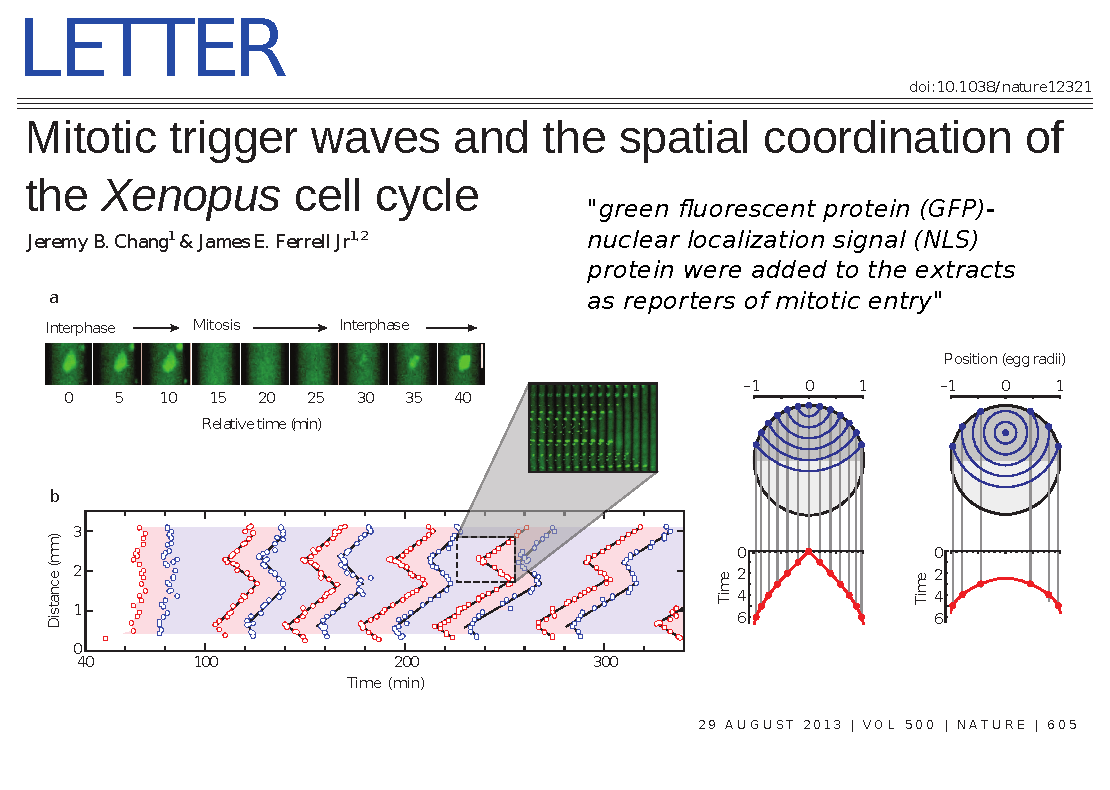
\includegraphics[width=0.8\textwidth]{chang.eps}
	\frametitle{Kémiai hullámok \emph{Xenopus} embrióban}
\end{frame}

\begin{frame}
	\centering
	\includegraphics[width=0.8\textwidth]{setup1.jpg}
	\frametitle{Pontszerű mérés}
	\framesubtitle{Módszer}
\end{frame}


\begin{frame}
\frametitle{Pontszerű mérés}
\framesubtitle{A mért paraméterek}
\begin{columns}[T] % align columns
\begin{column}{.48\textwidth}

\centering
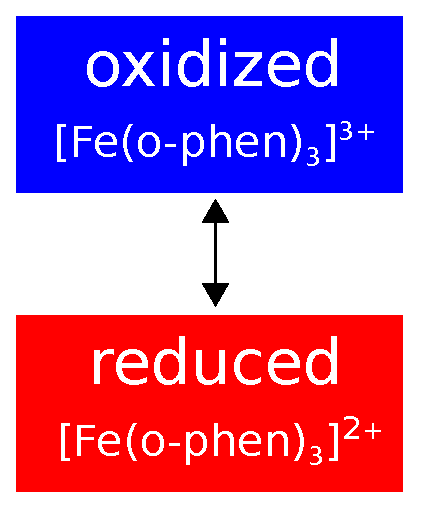
\includegraphics[width=0.6\textwidth]{ferroin.eps}

Ferroin redox--indikátor

\end{column}%
\hfill%
\begin{column}{.48\textwidth}
%\color{blue}\rule{\linewidth}{4pt}
\centering


%\footnotesize
\begin{equation*}
        E=E^\theta + \frac{RT}{z_iF} \ln \frac{[Fe^{3+}]}{[Fe^{2+}]}
\end{equation*}
%\normalsize

Nernst--egyenlet
\end{column}%
\end{columns}
\end{frame}


\begin{frame}
	\centering
	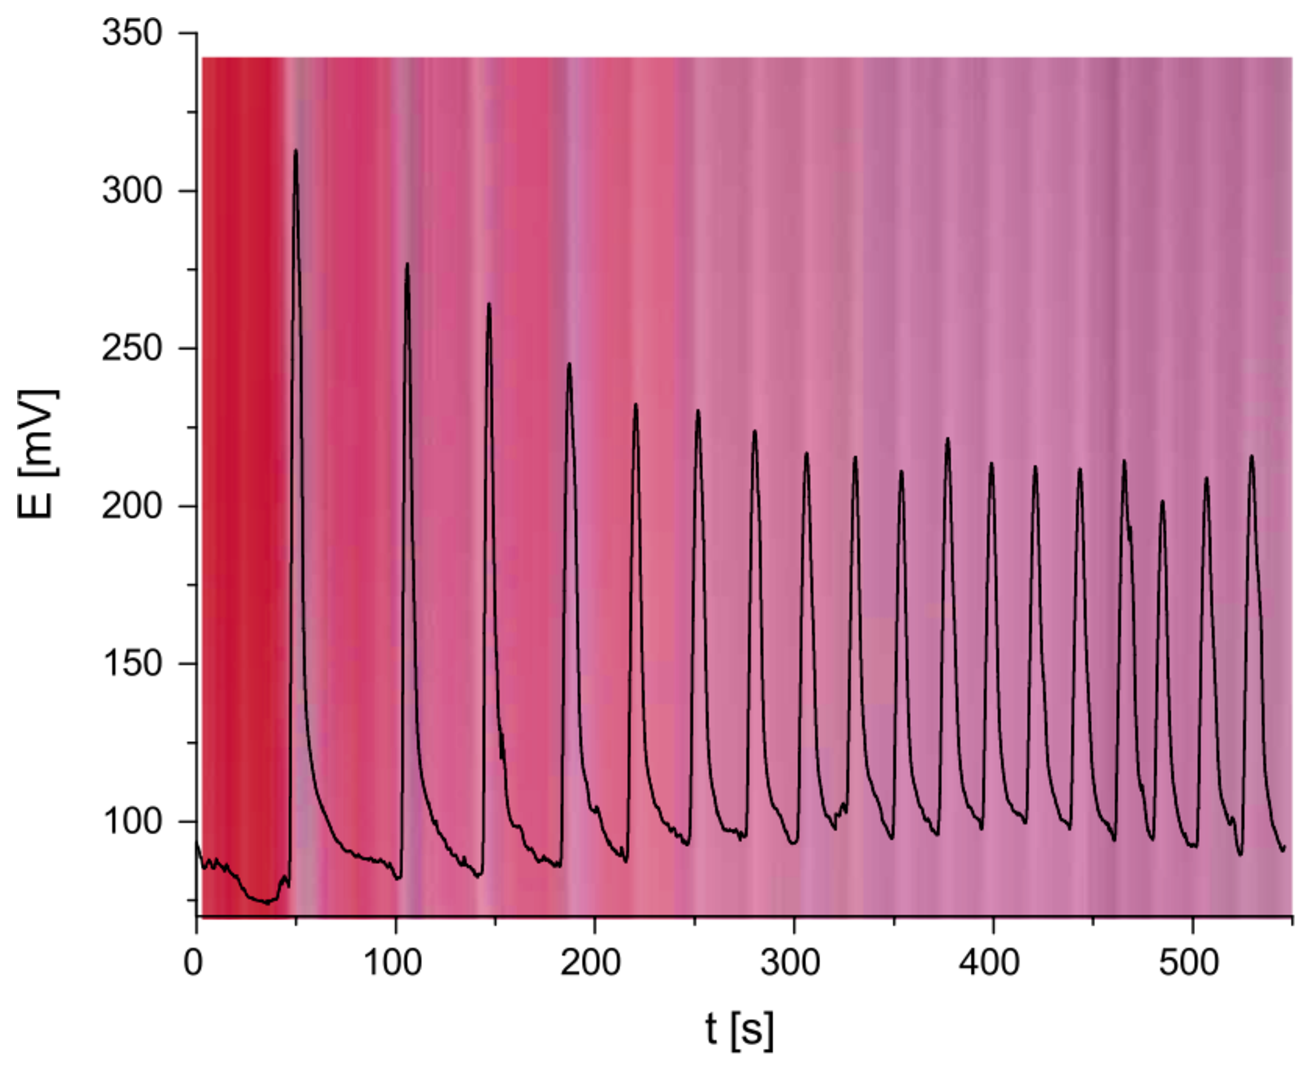
\includegraphics[width=0.8\textwidth]{pontszerumeres.eps}
	\frametitle{Pontszerű mérés}
	\framesubtitle{Eredmény}
\end{frame}



\begin{frame}
	\centering
	\includegraphics[width=0.8\textwidth]{setup_photo.jpg}
	\frametitle{PEKM pásztázás}
	\framesubtitle{Mérési elrendezés fotója}
\end{frame}

\begin{frame}
	\centering
	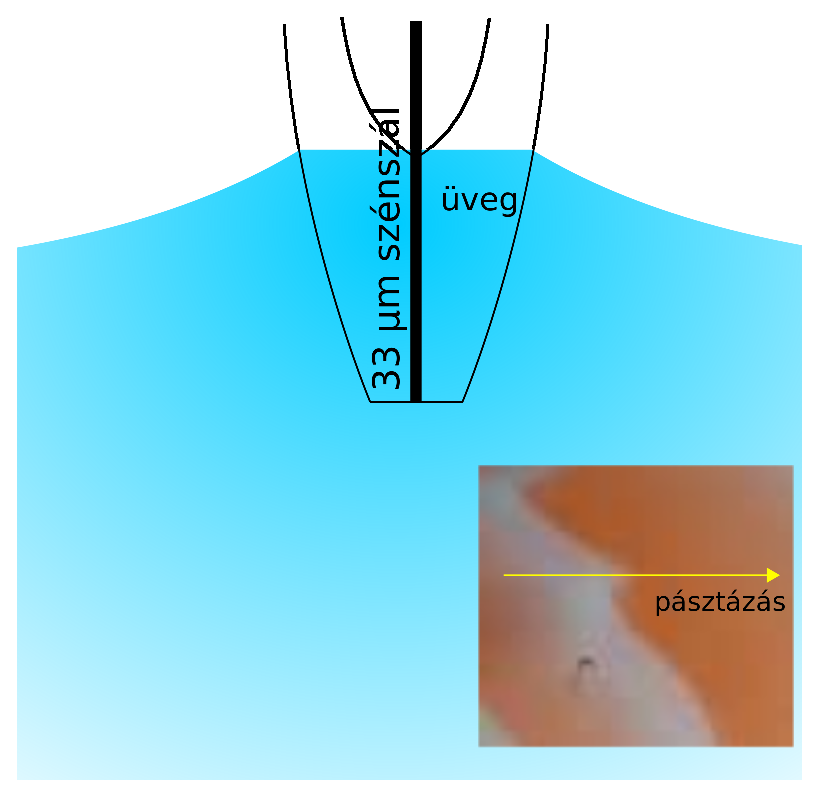
\includegraphics[width=0.6\textwidth]{szigeteles1.eps}
	\frametitle{Konvektív zavarás}
	\framesubtitle{Konvencionális szénszál mikroelektród a reakcióelegyben}
\end{frame}

\begin{frame}
	\centering
	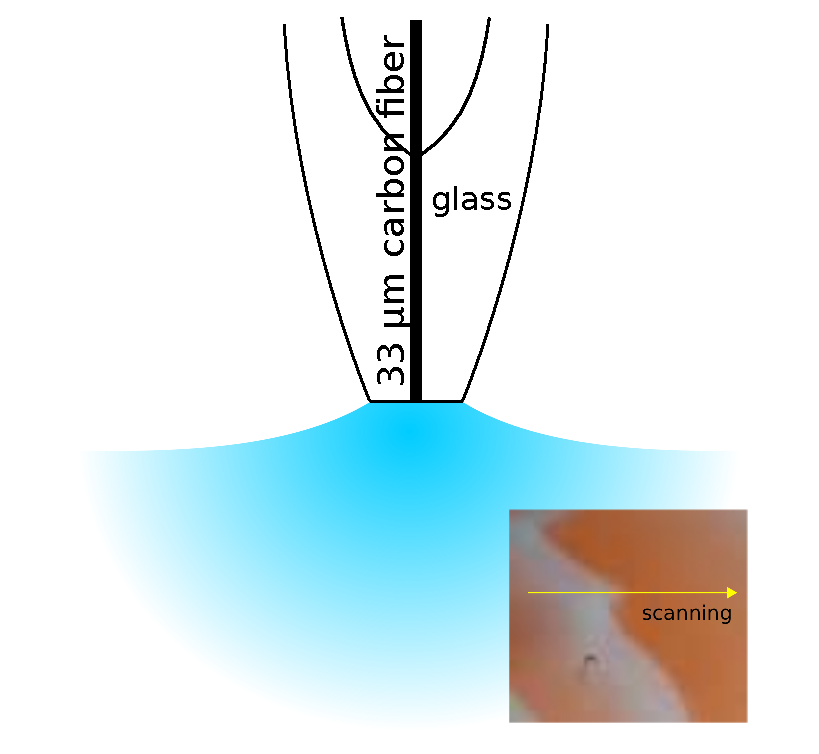
\includegraphics[width=0.6\textwidth]{szigeteles2.eps}
	\frametitle{Konvektív zavarás}
	\framesubtitle{Konvencionális szénszál mikroelektród a reakcióelegy felületén}
\end{frame}

\begin{frame}
	\centering
	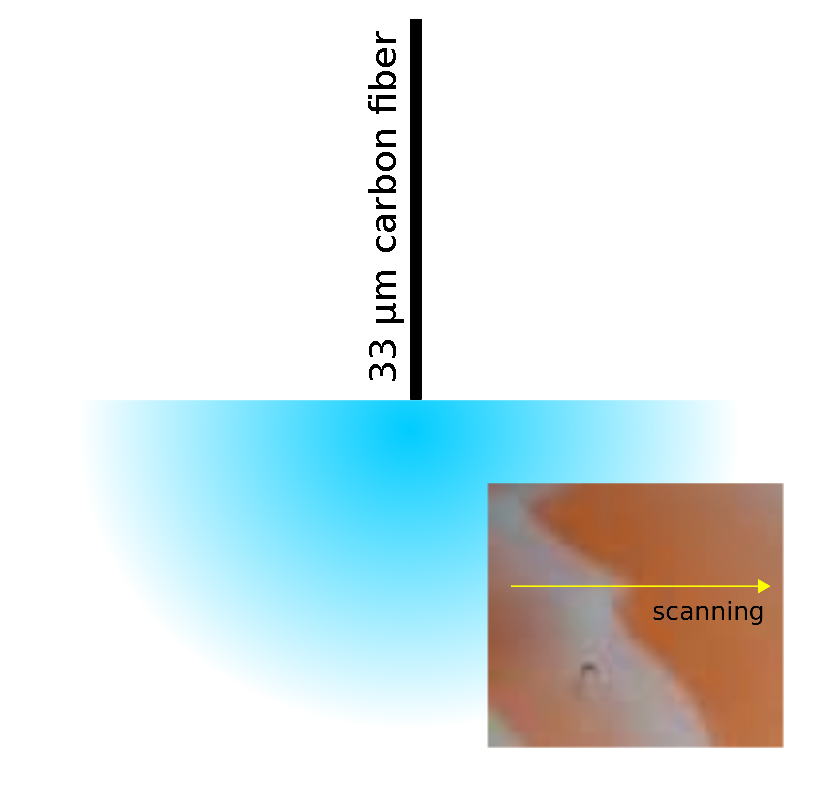
\includegraphics[width=0.6\textwidth]{szigeteles3.eps}
	\frametitle{Konvektív zavarás}
	\framesubtitle{Szigetelés nélküli szénszál mikroelektród a reakcióelegy felületén (d = 33 $\upmu$m)}
\end{frame}

\begin{frame}
	\centering
	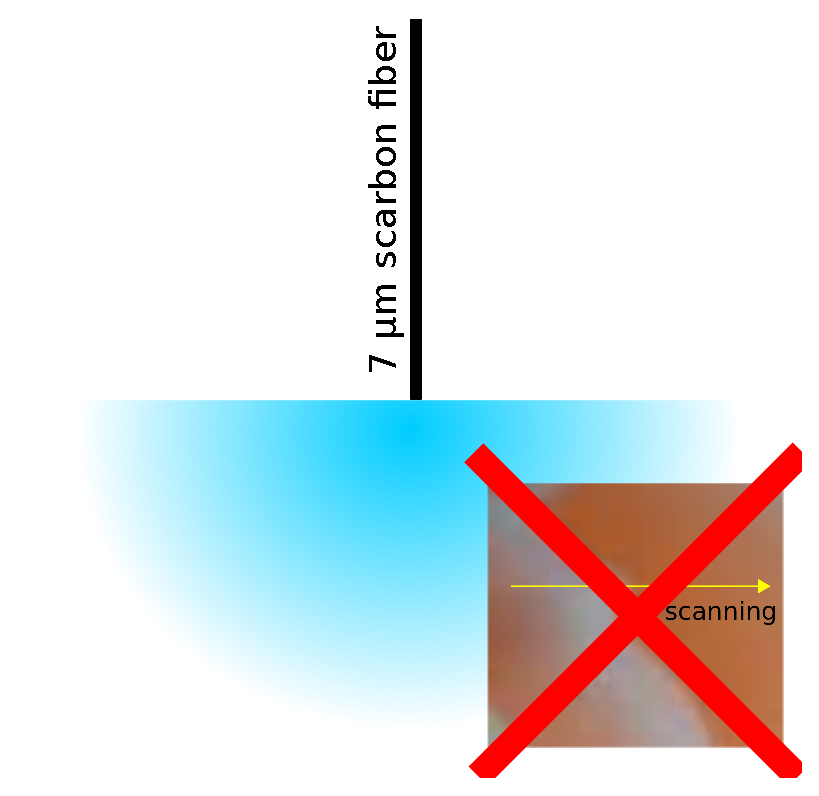
\includegraphics[width=0.6\textwidth]{szigeteles4.eps}
	\frametitle{Konvektív zavarás}
	\framesubtitle{Szigetelés nélküli szénszál mikroelektród a reakcióelegy felületén (d = 7 $\upmu$m)}
\end{frame}

\begin{frame}
	\centering
	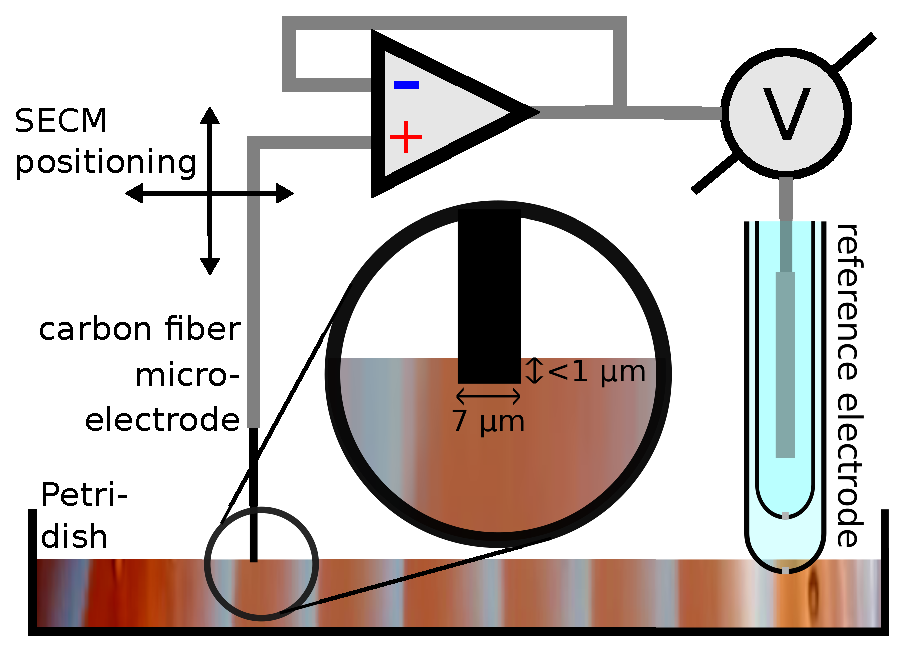
\includegraphics[width=0.8\textwidth]{setup.eps}
	\frametitle{PEKM pásztázás}
	\framesubtitle{Mérési elrendezés sematikus ábrája}
\end{frame}

\begin{frame}
	\centering
	\includegraphics[width=0.6\textwidth]{grabs.png}
	\frametitle{PEKM pásztázás}
	\framesubtitle{Konvekciós zavarás vizsgálata}
\end{frame}

\begin{frame}
	\centering
	\includegraphics[width=0.8\textwidth]{spacetime_ill.eps}
	\frametitle{PEKM pásztázás}
	\framesubtitle{Mérés kiértékelése}
\end{frame}

\begin{frame}
	\centering
	\includegraphics[trim = 15mm 60mm 0mm 30mm, clip, width=0.5\textwidth, angle=-90]{spacetime.eps}
	\frametitle{PEKM pásztázás}
	\framesubtitle{Eredmény}
\end{frame}

\begin{frame}
	\frametitle{PEKM pásztázás}
	\framesubtitle{Eredmény}

\begin{table}
\tiny
\label{table:stats}
\centering
\begin{tabular}{r c c c c c}
Wave \# & t, s & E, mV & x, mm & v, $\upmu$m/s \\
 \hline
 \hline
 3&\begin{tabular}{c}47\\67\\80\end{tabular}&\begin{tabular}{c}957\\978\\977\end{tabular}&\begin{tabular}{c}1.4\\6.4\\8.6\end{tabular}&218.8\\
 \hline
 6&\begin{tabular}{c}99\\114\\133.5\end{tabular}&\begin{tabular}{c}968\\975\\1027\end{tabular}&\begin{tabular}{c}1\\4.8\\7.6\end{tabular}&191.3\\
 \hline
 7&\begin{tabular}{c}148.5\\171\\181.5\end{tabular}&\begin{tabular}{c}1052\\1127\\1059\end{tabular}&\begin{tabular}{c}1.6\\7.2\\8.8\end{tabular}&218.18\\
 \hline
 9&\begin{tabular}{c}200\\219.5\\234.5\end{tabular}&\begin{tabular}{c}1016\\1074\\1016\end{tabular}&\begin{tabular}{c}1.4\\6.2\\8\end{tabular}&191.3\\
 \hline
 12&\begin{tabular}{c}253.5\\268\\287\end{tabular}&\begin{tabular}{c}1060\\1120\\1053\end{tabular}&\begin{tabular}{c}0.4\\5.2\\7.4\end{tabular}&208.96\\
\end{tabular}
\end{table}
\end{frame}


\begin{frame}
	\frametitle{Összefoglalás}
	\centering
\begin{itemize}
\item Megfelelően kis átmérőjű mikroelektród mozgás közben sem zavarja a BZ--reakciót.

\item PEKM technikával ötvözhetők az optikai és az elektrokémiai módszerek előnyei a BZ-reakció vizsgálatához, és térbeli felbontású kémiai információ nyerhető a reakcióról.

\item A mérőcsúcs kicserélésével hasonló módon térképezhető lenne a pH és bromid-ion aktivitás.

\item A folyadékfázis felületi pásztázása más esetekben is alkalmazható lehet.
\end{itemize}
\end{frame}


\begin{frame}
	\centering
	Köszönettel tartozom doktori témavezetőmnek,\\ Nagy Géza professzor Úrnak \\ és a tanszék minden dolgozójának, \\ akik munkámban segítettek.
\end{frame}

\begin{frame}
	\centering
	Köszönöm a megtisztelő figyelmüket.

%	\includegraphics[width=0.8\textwidth]{thanks.jpg}

\end{frame}



\end{document}
